\section*{Question 8}
\textit{Plot the pre-multiplied spectrum for both datasets and calculate the dominant time-scale (and hence length scale using Taylor’s hypothesis) using this data by locating the peak in this pre-multiplied spectrum.}

\begin{figure}[!ht]
\centering
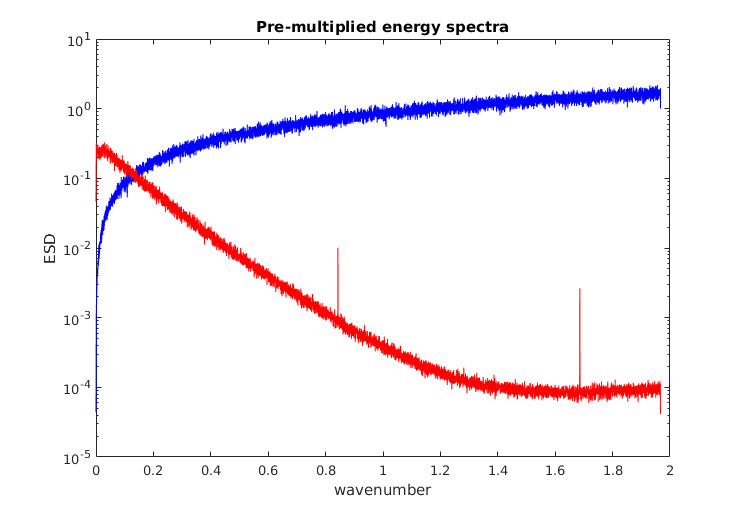
\includegraphics[scale=0.8]{./TEXT/esd-n.png}
\caption{Comparison between the pre-multiplied energy spectral densities in the spatial domain of both flow cases as they change with wave-number for a window size of $20'000$ data points}
\label{esd-n}
\end{figure}

The dominant time scale is given by finding the index of the maximum value of the pre-multiplied spectrum and using it to choose the corresponding wave-number. The length scales for flows 1 and 2 are $\sim 2 m$ and $4.58 \times 10^{-3} m$ respectively. When compared to the $T_{int}$ values in table \ref{scales} they differ to a large degree especially for \emph{flow 1}. In the second case the difference is not very large given the different approaches taken and they seem to be reasonable if they are thought of as describing a range for the sizes of the eddies that carry the largest part of the kinetic energy.